%% The following is a directive for TeXShop to indicate the main file
%%!TEX root = diss.tex

\chapter{A Taxonomy of 3D Reconstruction}
\label{ch:3DRecon_Taxo}
Existing taxonomies of 3D reconstruction techniques generally focus on one category of techniques: the Multi-view Stereo taxonomy in~\cite{seitz2006comparison} proposed classification of MVS algorithms from various perspectives. Reviews of Structured Light techniques generally classify techniques based on the type of projection pattern used~\cite{geng2011structured, salvi2004pattern}. Photometric Stereo algorithms are classified by the assumptions or generalizations made, for instance, unknown/known reflectance, unknown/known light conditions (uncalibrated/calibrated), etc~\cite{shi2016benchmark}. These frameworks provide a way to categorize intra-category algorithms, but is unsuitable to evaluate the performance of inter-category algorithms. Furthermore, the algorithms under consideration are targeted at a limited categories of objects. It's well known that these algorithms are highly likely to fail on other categories of objects, and this knowledge of algorithmic applicability is largely empirical, with each algorithm roughly maps to a problem domain that is poorly defined. Thus we need a more object-centered approach to the taxonomy so that a more precise mapping is available.

It's crutial to understand where algorithms perform well and where they fail when designing an application for reconstruction. Under the previous framework of taxonomy, this knowledge is largely empirical, with each algorithm mapped roughly to a sub-volume in the problem space. However, this mapping is ambigueous, \ie the sub-space is not well defined, and also too general, \ie algorithm within the same category cannot be effectively distinguished. To overcome this limitation, we need to 1). propose a well-defined problem space; 2). bypass the algorithmic details and focus on properties that are not intuitive to understand and perceive.

The taxonomy proposed in this chapter defines the 3D reconstruction techniques from an object-centered viewpoint, \ie categorize algorithm based on object class. This taxonomy transforms the 3D reconstruction problem from one requiring knowledge and expertise of specific algorithms in terms of how and when to use them, to one requiring knowledge of the visual and geometric properties of the target object.

\section{A New Perspective of Taxonomy}
Typical taxonomies generally focus on one class of algorithms, and are algorithm centric, describing and classifying intra-class algorithms based on \textit{how} an algorithm solves the problem. However, this approach 1). gives very little insight to what conditions does a specific algorithm work well; 2). requires vision knowledge to understand and use these algorithms. The new taxonomy approaches this problem from a different perspective, more specifically, the algorithms are categorized based on the type of objects/problem conditions that they can reliably work under. We first give an overview of object classes, which serves as the bases to the taxonomy.

\subsection{Object class}
In Figure~\ref{fig:obj_class} (a), we show a taxonomy of object classes with different material and shape properties. There are in total $3\times 3\times 2\times4\times 2\times 5 = 720$ classes of objects, which still don't fully capture the variations exhibited by real world objects, for instance, effects such as occlusion, discontinuity, emission, etc are not considered.
\begin{figure}[!htbp]
\centering
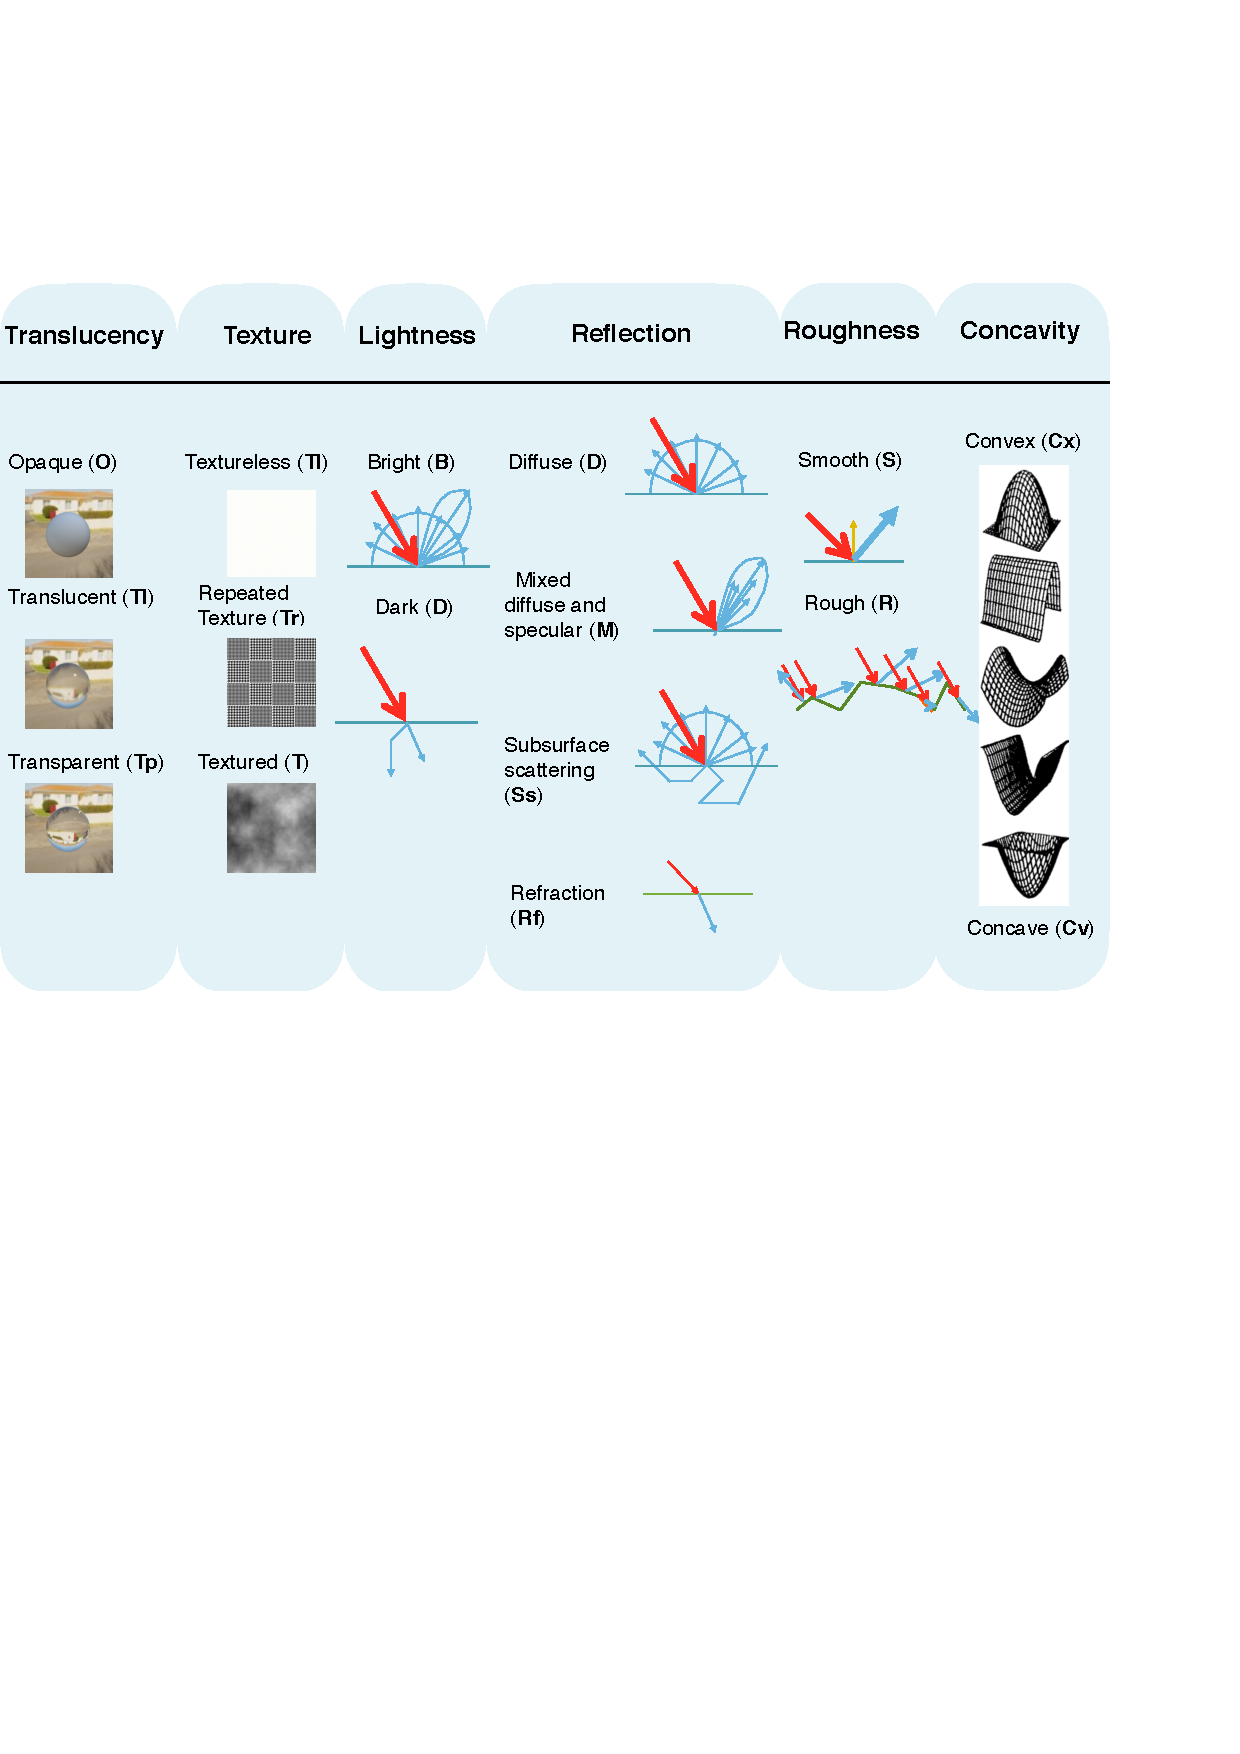
\includegraphics[width=0.8\textwidth]{taxo/obj_class}\\
\caption{A list of properties for object classes.}
\label{fig:obj_class}
\end{figure}

\subsection{Class labels}
We propose the following labels to the differentiate object classes reviewed above. The order of the labels are: translucency, texture, lightness, reflection model, surface roughness, and concavity.
\begin{itemize}
\item \textbf{Translucency}: \textbf{O}: opaque, \textbf{Tl}: translucent, \textbf{Tp}: transparent.
\item \textbf{Texture}: \textbf{T}: textured, \textbf{Tr}: repeated textured, \textbf{Tl}: textureless.
\item \textbf{Lightness}: \textbf{B}: bright, \textbf{D}: dark.
\item \textbf{Reflection}: \textbf{D}: diffuse model, \textbf{S}: specular model, \textbf{M}: mixture of diffuse and specular, \textbf{Ss}: subsurface scattering, \textbf{Rf}: refraction
\item \textbf{Roughness}: \textbf{S}: smooth, \textbf{R}: rough
\item \textbf{Concavity}: \textbf{Cx}: convex, \textbf{Cv}: concave
\end{itemize}

Most techniques that have been developed over the past decades can only tackle a subset of all possible object classes, with a focus on opaque, diffuse objects. For specular, refractive, and translucent or transparent objects, only very specialized algorithms are applicable for reconstruction~\cite{ihrke2010transparent}. Therefore, we consider only the six classes of objects listed in Table~\ref{tab:six_obj_class}.
\begin{table}[!htbp]
\centering
\begin{tabular}{l|*{6}{c}}
\toprule
Class \# & Translucency & Texture & Lightness & Refection & Roughness & Concavity\\
\midrule
1 & O & Tl & B & D & R & Cx\\
2 & O & Tl & B & M & S & Cx\\
3 & O & T & B & D & R & Cx\\
4 & O & T & B & M & S & Cx\\
5 & O & T & D & D & S & Cx\\
6 & O & T & D & M & S & Cx\\
\bottomrule
\end{tabular}
\caption{Label of the six classes of objects.}
\label{tab:six_obj_class}
\end{table}

\subsection{Classes of algorithms}
Here is a list of seletected algorithms that will be looked into in depth, a summary is list in Figure~\ref{tab:class_algo}.
\begin{table}[!htbp]
  \centering
  \begin{tabular}{l|l}
  \toprule
  \textbf{Algo. class} & \textbf{Technique}\\
  \midrule
  SfS & Horn~\cite{horn1970shape}\\
  MVS & Furukawa~\cite{furukawa2010accurate}, Goesele~\cite{goesele2006multi}, Vogiatzis~\cite{vogiatzis2007multiview}, \\
      & Hern{\'a}ndez~\cite{esteban2004silhouette}, Faugeras~\cite{faugeras2002variational}\\
  Lamberian PS & Woodham~\cite{woodham1980photometric}, Hayakawa~\cite{hayakawa1994photometric}, Belhumeur~\cite{belhumeur1999bas}, \\
      & Alldrin~\cite{alldrin2007resolving}\\
  Non Lambertian PS & Coleman~\cite{coleman1982obtaining}, Barsky~\cite{barsky20034}, Schluns~\cite{schluns1993photometric}, Sato~\cite{sato1994temporal}, \\
      & Mallick~\cite{mallick2005beyond}, Alldrain~\cite{alldrin2008photometric}, Goldman~\cite{goldman2010shape}, Silver~\cite{silver1980determining}, \\
      & Hertzmann~\cite{hertzmann2005example}, Zickler~\cite{zickler2002helmholtz}\\
  % MVPS & \checkmark & \\
  SL & Inokuchi~\cite{inokuchi1984range}\\
  VH & Szeliski~\cite{szeliski1993rapid}, Matusik~\cite{matusik2002efficient}, Tarini~\cite{tarini2002marching}\\
  \bottomrule
  \end{tabular}
  \caption{Selected algorithms from each class of algorithms}
  \label{tab:class_algo}
\end{table}

\section{Working conditions of algorithms}
This section investigate the cases where each categories of algorithm is capable to work under based on the reported literature.

\subsection{Multi-view Stereo}
The working conditios of Multi-view Stereo algorithms are summarized in Table~\ref{tab:mvs_cond}.

\subsubsection{High texture}
Multi-view Stereo algorithms take advantage of the textural information to establish point correspondences across various viewpoints, thus they work best under high textured conditions.

% \citeauthor{furukawa2008high} use wide-baseline stereo matching to recover the 3D coordinates of salient feature points, then shrink a visual hull model so that the recovered points lie on its surface, then refine the result using energy minimization. \citeauthor{goesele2006multi} compute a depth map from each camera viewpoint (similar to [31]) and merge the results using VRIP [62]. \citeauthor{esteban2004silhouette} first compute a depth map from each camera viewpoint and merge the results into a cost volume. They then iteratively deform a mesh, initialized at the visual hull, to find a minimum cost surface in this volume, also incorporating terms to fit silhouettes. Kolmogorov and Zabih [35] compute a set of depth maps using multi-baseline stereo with graph cuts, then merge the results into a voxel volume by computing the intersections of the occluded volumes from each viewpoint. \citeauthor{faugeras2002variational} compute a minimum cost surface by evolving a surface in a level-set frame-work, using a prediction-error measure. \citeauthor{vogiatzis2007multiview} compute a correlation cost volume in the neighborhood of the visual hull. A minimum-cost surface is then computed using volumetric min-cut.

\subsubsection{Diffuse reflectance}
Most MVS algorithms require that the matching image region with similar or same appearances from different angles, and hence, most of the algorithms assume Lambertian reflectance. While pure Lambertian surfaces are rare in practice, it is known and empirically verified that MVS algorithms work very well on non-Lambertian surface: as long as they contain some diffuse reflectance component, and the photo-consistency function is able to identify and ignore images whose non-diffsue effects(e.g., specular highlights) are strong, then utilize the diffuse component in the remaining images. However, there are some attempts to overcome this limitations, a pure passive methods was proposed that directly model and analyze non-Lambertian effects for MVS algorithms~\cite{jin2003multi,jin2005multi}.
\begin{table}[!htbp]
  \centering
  \begin{tabular}{l*{5}{p{15mm}}}
  \toprule
  \textbf{Technique} & Texture & Lightness & Reflectance & Roughness & Concavity\\
  \midrule
  MVS & Textured & - & Diffuse or mixed & - & -\\
  \bottomrule
  \end{tabular}
  \caption{Working conditions of typical Multi-view Stereo algorithms.}
  \label{tab:mvs_cond}
\end{table}

\subsection{Shape from Shading}
Shape from Shading, first proposed by~\citeauthor{horn1970shape} is targeted specifically for known isotropic Lambertian surfaces. By assuming orthographic projection, and known light source intensity and direction, surface orientation can be estimated from the shading variations. The working condition is shown in Table~\ref{tab:sfs_cond}.
\begin{table}[!htbp]
  \centering
  \begin{tabular}{l*{5}{p{15mm}}}
  \toprule
  \textbf{Technique} & Texture & Lightness & Reflectance & Roughness & Concavity\\
  \midrule
  SfS & Textureless & Bright & Lambertian & - & Convex\\
  \bottomrule
  \end{tabular}
  \caption{Working conditions of typical Shape from Shading algorithms.}
  \label{tab:sfs_cond}
\end{table}

\subsection{Photometric Stereo}
The working conditions of Photometric Stereo algorithms are presented below. Visual texture can be thought of as a pattern or variance of intensity appearing on an object's surface. In this thesis, the visual texture will be considered as resulting from non-uniform surface albedo. Thus uniform albedo represents uniform texuture while non-uniform albedo represents textured surface. The working conditions are shown in Table~\ref{tab:ps_cond}.

\subsubsection{Albedo}
Photometric Stereo can only work well on surfaces with high albedo.

The original PS was developed for surfaces with uniform albedo, PS can be extended easily for spatially varying albedo. First the albedo-scaled normal can be first estimated as usual, then the albedo is retrieved as the magnitude of the scaled normal~\cite{woodham1980photometric}.

\subsubsection{Lambertian reflectance} % Lambertian PS: uniform reflectance
The traditional Photometric Stereo can be considered as an extenstion of the original Shape from Shading, which incorporates additional light sources to eliminate ambiguity~\cite{woodham1980photometric}, thus are only applicable to Lambertian surface with uniform albedo.

To avoid the tedious process of light calibration, Silver~\cite{silver1980determining} proposed a look-up table scheme that relies on reflectance object with the same reflectance as the target, a uniform Lambertian surface in this case. This approach is later adapted to surface with non-Lambertian reflectance with varying albedo or material in~\cite{hertzmann2005example}.

The original Photometric Stereo require light calibration, \textit{uncalibrated photometric stereo} has been proposed to avoid this tedious process. One approach used six or more pixels with the same albedo, and was able to solve for normals up to a rotation ambiguity\cite{hayakawa1994photometric}. It can be further proved that a 3-parameter subset of these transformations, known as the Generalized Bas-Relief (GBR) ambiguity, preserve surface integrability~\cite{belhumeur1999bas}. Thus, given three or more imges of a Lambertian object acquired under light sources of unknown direction and strength, the surface can be reconstructed up to GBR transformation by enforcing surface integrability, see Figure~\ref{fig:gbr} for the effect of GBR-ambiguity.
\begin{figure}[!htbp]
\centering
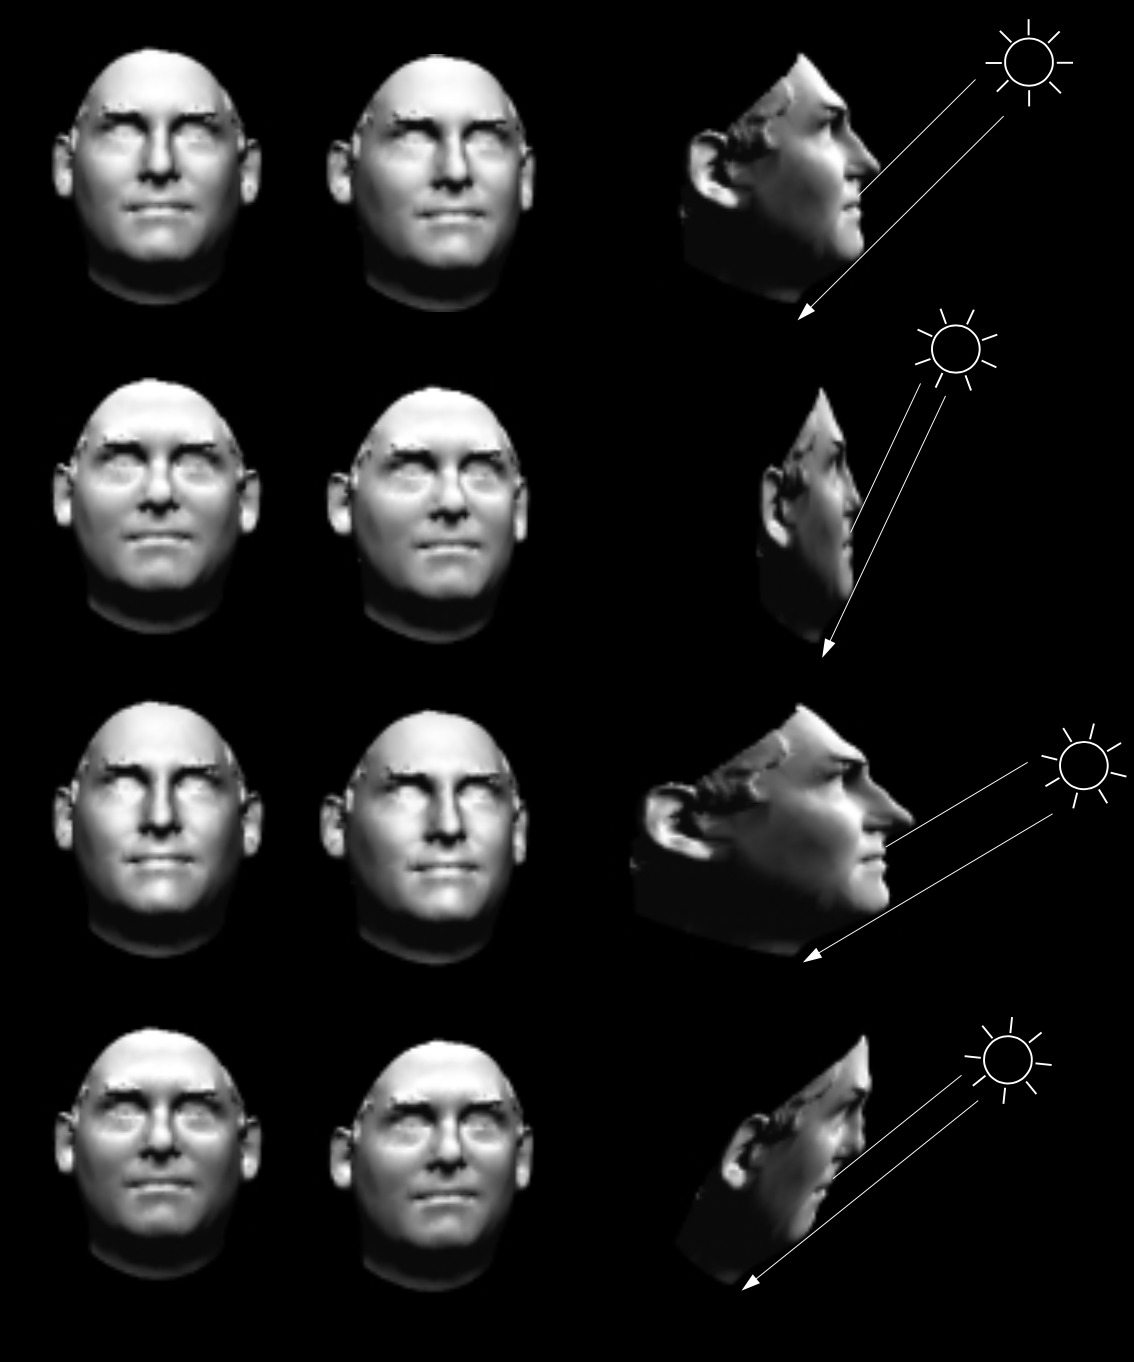
\includegraphics[width=0.6\textwidth]{taxo/gbr.png}
\caption{The effect of GBR ambiguity}
\label{fig:gbr}
\end{figure}

\subsubsection{Non-Lambertian reflectance}
The \textit{reference object} approach, first proposed by~\citeauthor{silver1980determining}, and later revisited by in~\cite{hertzmann2005example}, can be used for surfaces with spatially varying reflectance. The basic assumption is that the BRDF at each point is a linear combination of the ``basis'' BRDFs defined by the set of reference objects.

One approach exploits the fact that the reflectance of non-Lambertian surfaces can be approximated by \textbf{diffuse component and specular lobe}. \citeauthor{coleman1982obtaining} and \citeauthor{barsky20034} who treat specular pixels as outliers, and \citeauthor{schluns1993photometric}, \citeauthor{sato1994temporal}, and \citeauthor{mallick2005beyond} who assume the color of the specular lobe differs from the color of the diffuse lobe, allowing separation of the specular and diffuse components.

Due to the high complexity of the BRDF, some methods utilize {analytical reflectance models}. \citeauthor{goldman2010shape} uses an isotropic Ward model for each basis BRDF, and the surface orientation and parameters of the reflectance models are estimated iteratively. \citeauthor{alldrin2008photometric} proposed a data-driven approach that got rid of the parametric reflectance model, and employed an novel bi-variate approaximations of isotropic reflectance functions. By combining this approximation with the weighted basis BRDFs, a per-pixel surface normal, global set of non-parametric basis BRDFs, and the corresponding weights are able to be independently estimated. Though the parametric reflectance model can significantly reduce the complexity of BRDFs, they are typically restricted to a limited classes of materials.

Another alternative to using BRDF models is to take advantage of the properties of BRDFs, include energy conservation, non-negativity, Helmholtz reciprocity, or isotropy. Helmholtz stereopsis introduced by~\citeauthor{zickler2002helmholtz} exploits the reciprocity to obtain the surface reconstruction. Isotropy is another physical property which holds for material without ``grain''. \citeauthor{tan2007isotropy} use both symmetry and reciprocity present in isotropic BRDFs to resolve the generalized bas-relief ambiguity. \citeauthor{alldrin2007toward} show that isotropy, with no further assumptions on surface shape or BRDF, can be utilized to recover the surface normal at each surface point up to a plane.
% A four-source photometric stereo technique uses a fourth source of illumination to detecta and remove specular reflections~\cite{coleman1982obtaining}. By adding a fourth image, it's possible to compute four sets of normals, \ie one normal for each permutation of three intensity values. If there is a greater deviation in both magnitude and direction of the normals, a method can now be developed to eliminate specular effects using a thresholding procedure.

\subsubsection{Convex}
Active methods that assumes a local reflectance model such as most PS can work more reliably for surfaces without casting shadow. Thus the concave surfaces pose a great challenge for this technique since the indensity is no longer determined solely by the light source, surface normal and viewing direction.
\begin{table}[!htbp]
  \centering
  \begin{tabular}{p{3cm}*{5}{p{15mm}}}
  \toprule
  \textbf{Technique} & Texture & Lightness & Reflectance & Roughness & Concavity\\
  \midrule
  Lambertian PS, uniform albedo & Textureless & Bright & Lambertian & - & Convex\\
  Lambertian PS, non-uniform albedo & Textured & Bright & Lambertian & - & Convex\\
  Non-Lambertian PS, uniform albedo & Textureless & Bright & Mixed & - & Convex\\
  Non-Lambertian PS, non-uniform albedo & Textureled & Bright & Mixed & - & Convex\\
  \bottomrule
  \end{tabular}
  \caption{Working conditions of typical Photometric Stereo algorithms.}
  \label{tab:ps_cond}
\end{table}

\subsection{Structured Light}
For stereo correspondence based methods, actively projected patterns have to be used for the lack of surface texture. Since the surface is diffuse, there is no specular reflection to cause severe noise. Refer to Table~\ref{tab:sl_cond} for the working condition of SL.
\subsubsection{High albedo}
The surface should be sufficiently light, otherwise, the lit areas would be erreneously decoded as unlit, causing correspondence errors.

\subsubsection{Diffuse reflectance}
Traditional Structured Light techniques don't cope well with highly specular surface since the pattern is undistinguishable at areas with specular highlights.

\subsubsection{Concex}
Active methods that assumes a local reflectance model such as most PS can work more reliably for surfaces without casting shadow. Thus the concave surfaces pose a great challenge for this technique since the indensity is no longer determined solely by the light source, surface normal and viewing direction.
\begin{table}[!htbp]
  \centering
  \begin{tabular}{c*{5}{p{15mm}}}
  \toprule
  \textbf{Technique} & Texture & Lightness & Reflectance & Roughness & Concavity\\
  \midrule
  Structured Light & - & Bright & Lambertian & - & Convex\\
  \bottomrule
  \end{tabular}
  \caption{Working conditions of typical Structured Light algorithms.}
  \label{tab:sl_cond}
\end{table}

\subsection{Visual Hull}
Visual Hull algorithms don't rely on material properties as long as the foreground of the image can be reliably segmented, thus is applicable for all visual properties. However, it fails to carve out the concavities in the object, thus is unsuitable to high concave objects.
\begin{table}[!htbp]
  \centering
  \begin{tabular}{c*{5}{p{15mm}}}
  \toprule
  \textbf{Technique} & Texture & Lightness & Reflectance & Roughness & Concavity\\
  \midrule
  VH & - & - & - & - & Convex\\
  \bottomrule
  \end{tabular}
  \caption{Working conditions of typical Photometric Stereo algorithms.}
  \label{tab:ps_cond}
\end{table}
% \begin{table}[!htbp]
%   \centering
%   \begin{tabular}{l*{2}{c}}
%   \hline
%   \textbf{Technique} & Representation & Algorithm\\
%   \hline
%   Szeliski~\cite{szeliski1993rapid} & 3D grids & Voxel-based\\
%   Tarini~\cite{tarini2002marching} & 3D rays & MI-based\\
%   Matusik~\cite{matusik2002efficient} & Polygonal mesh & Exact polyhedral methods\\
%   \hline
%   \end{tabular}
%   \caption{Summary of VH representations and reconstruction approach.}
%   \label{tab:summary_class_6}
% \end{table}

\section{Summary}
Our taxonomy focuses on the visual cues detected in images, which is utilized by various techniques. Conceptualize these visual cues as dimension of the 3D reconstruction problem, we have an abstraction which allow us to think of algorithms as volumes within a $n-$dimensional problem space. Existing algorithms can be introduced into this framework based on the main visual cue used for reconstruction. Instances where these algorithms have been reported as supporting other forms of variation have been outlined, providing an initial mapping of the space that is summarized below in Table~\ref{tab:algo_taxo}.
\begin{figure*}[!htbp]
\centering
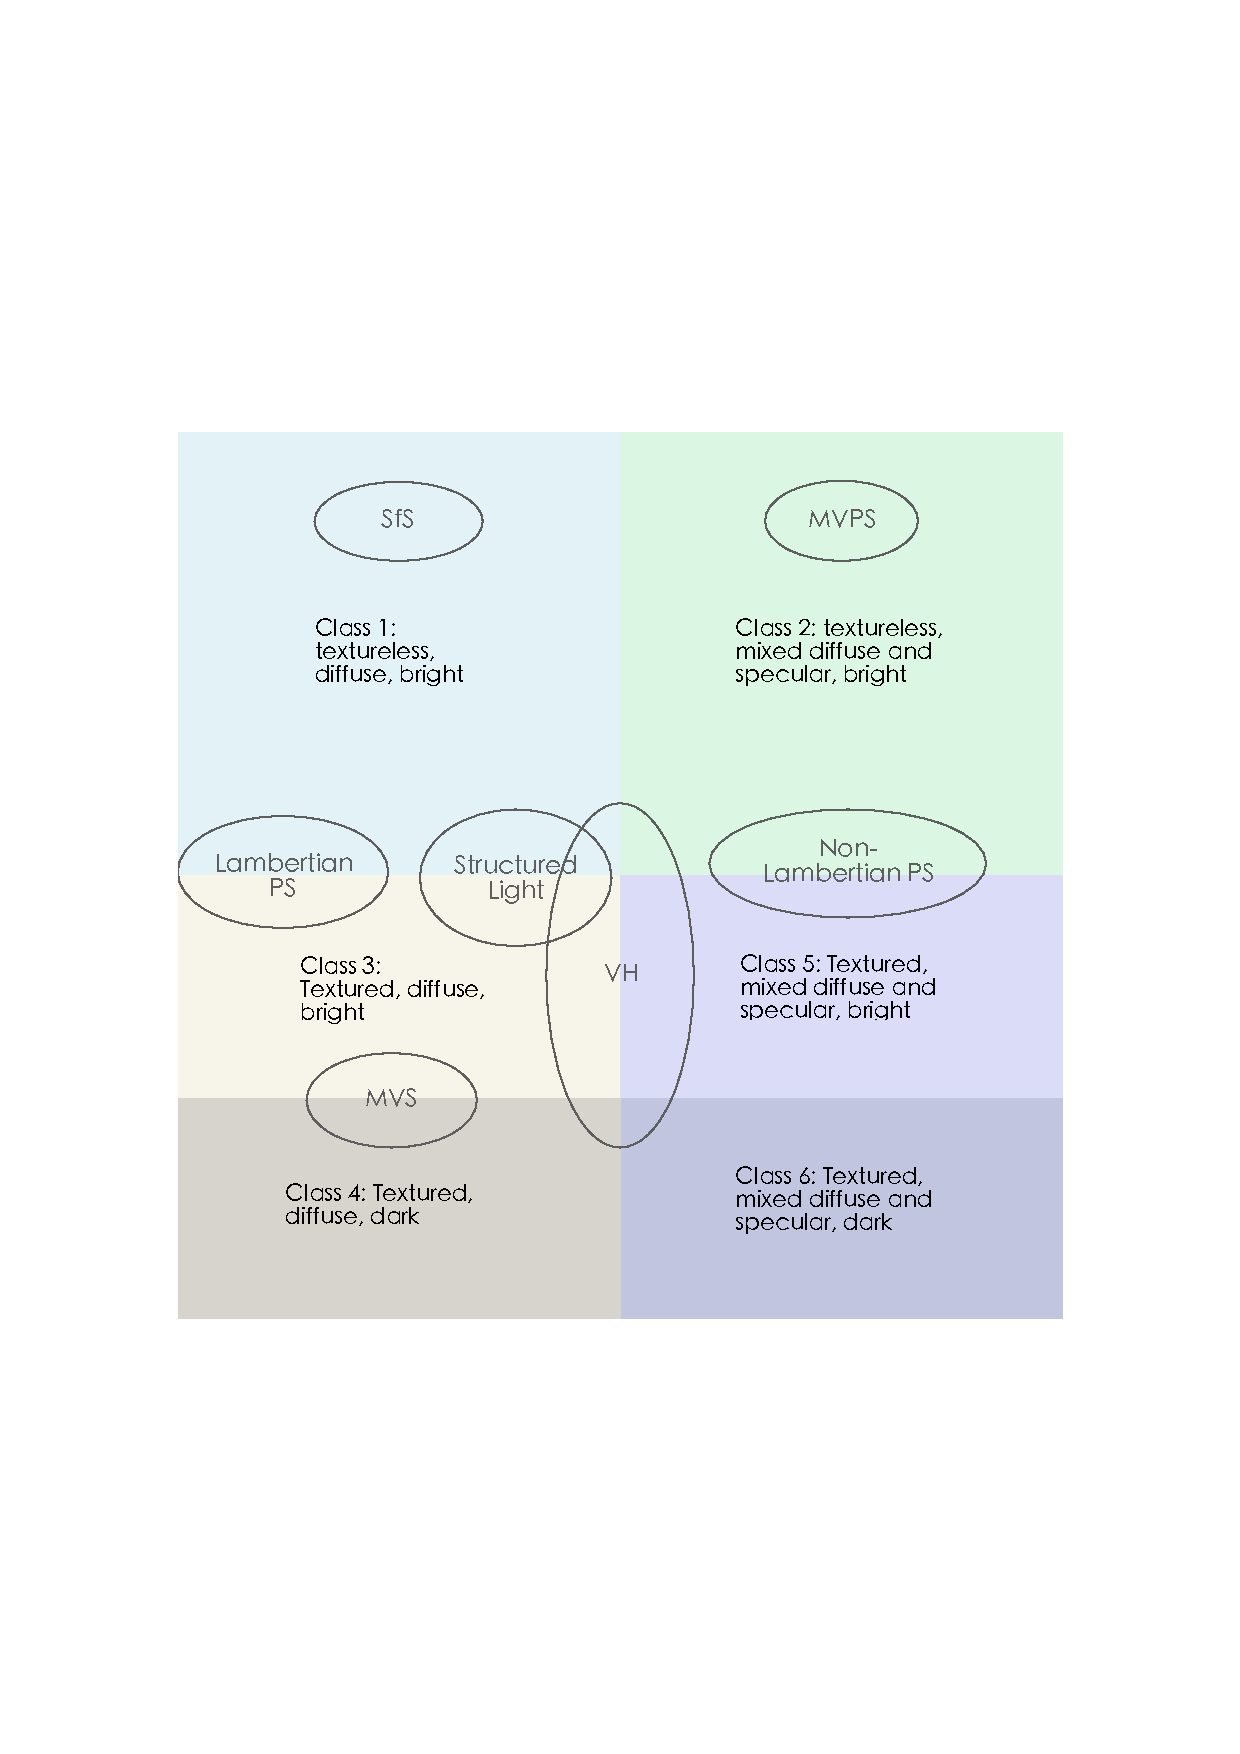
\includegraphics[width=0.5\textwidth]{taxo/six_class}
\caption{Six classes of objects of interest, and the algorithms that could work reliably for these classes.}
\label{fig:six_class}
\end{figure*}

\begin{table}[!htbp]
  \centering
  \begin{tabular}{l|p{10cm}}
  \toprule
  \textbf{Class \#} & Algorithms\\
  \midrule
  1 & Horn~\cite{horn1970shape}, Woodham~\cite{woodham1980photometric}, Hayakawa~\cite{hayakawa1994photometric}, Belhumeur~\cite{belhumeur1999bas}, Alldrin~\cite{alldrin2007resolving}\\
  2 & Coleman~\cite{coleman1982obtaining}, Barsky~\cite{barsky20034}, Schluns~\cite{schluns1993photometric}, Sato~\cite{sato1994temporal}, Mallick~\cite{mallick2005beyond}, Alldrain~\cite{alldrin2008photometric}, Goldman~\cite{goldman2010shape}, Silver~\cite{silver1980determining}, Hertzmann~\cite{hertzmann2005example}, Zickler~\cite{zickler2002helmholtz}\\
  3 & Woodham~\cite{woodham1980photometric}, Hayakawa~\cite{hayakawa1994photometric}, Belhumeur~\cite{belhumeur1999bas}, Alldrin~\cite{alldrin2007resolving}, Furukawa~\cite{furukawa2010accurate}, Goesele~\cite{goesele2006multi}, Vogiatzis~\cite{vogiatzis2007multiview}, Hern{\'a}ndez~\cite{esteban2004silhouette}, Faugeras~\cite{faugeras2002variational}, Inokuchi~\cite{inokuchi1984range}\\
  4 & Furukawa~\cite{furukawa2010accurate}, Goesele~\cite{goesele2006multi}, Vogiatzis~\cite{vogiatzis2007multiview}, Hern{\'a}ndez~\cite{esteban2004silhouette}, Faugeras~\cite{faugeras2002variational}\\
  5 & Coleman~\cite{coleman1982obtaining}, Barsky~\cite{barsky20034}, Schluns~\cite{schluns1993photometric}, Sato~\cite{sato1994temporal}, Mallick~\cite{mallick2005beyond}, Alldrain~\cite{alldrin2008photometric}, Goldman~\cite{goldman2010shape}, Silver~\cite{silver1980determining}, Hertzmann~\cite{hertzmann2005example}, Zickler~\cite{zickler2002helmholtz}\\
  6 & Szeliski~\cite{szeliski1993rapid}, Matusik~\cite{matusik2002efficient}, Tarini~\cite{tarini2002marching}\\
  \bottomrule
  \end{tabular}
  \caption{Algorithm classification based on the new taxonomy}
  \label{tab:algo_taxo}
\end{table}